\section{Results}
\label{sec:results}

\begin{figure*}[!ht]
 \centering
 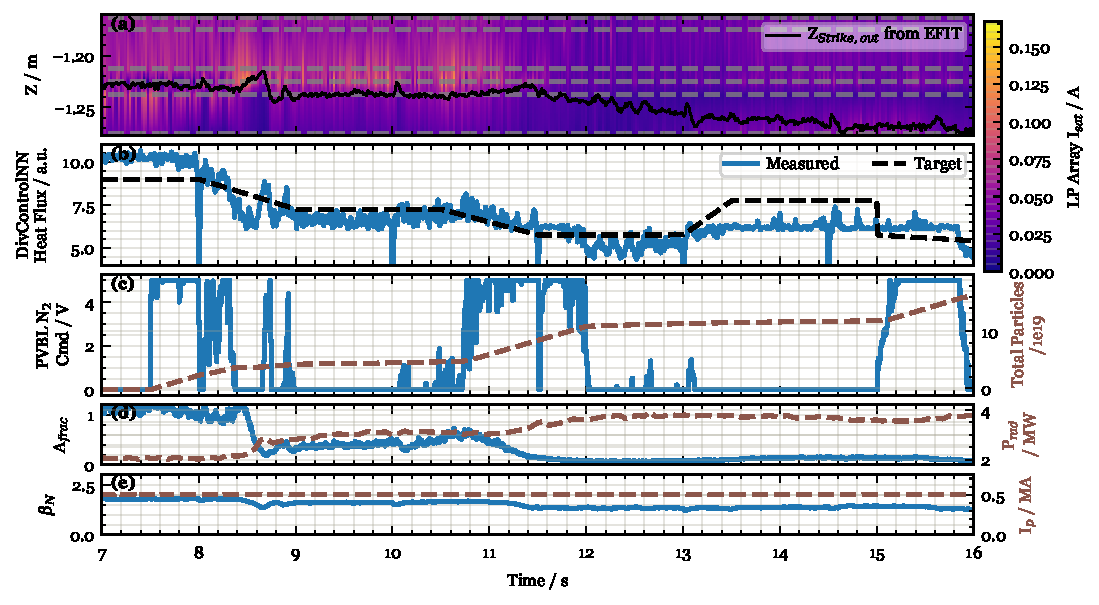
\includegraphics[width=\textwidth]{figures/DetCtrl_2D_36161.pdf}
 \caption{
Detachment control shot \# 36161 using DivControlNN heat flux at outer divertor.
(a) Shows the measured ion saturation current by realtime Langmuir Probe array at locations marked by grey dashed lines.
The data has been interpolated spatially using cubic spline interpolation.
The black curve shows the post-shot calculated strike point position on outer divertor using EFIT.
(b) Shows the heat flux at outer divertor calculated by DivControlNN.
The dashed black line shows the target provided to the controller to follow.
(c) Left axis: Shows the N$_2$ gas command steps sent for system identification.
Right axis: Shows the cummulative N$_2$ gas particles injected into the vessel.
(d) Left axis: Shows the \Afrac calculated from peak value among the Langmuir probe array.
Right axis: Total radiated power measured by \ac{IRVB}.
(e) Left axis: Shows $\beta_n$.
Right axis: Shows the plasma current (I$_p$).
}
 \label{fig:detctrl_sm}
\end{figure*}

\begin{figure}[!h]
 \centering
 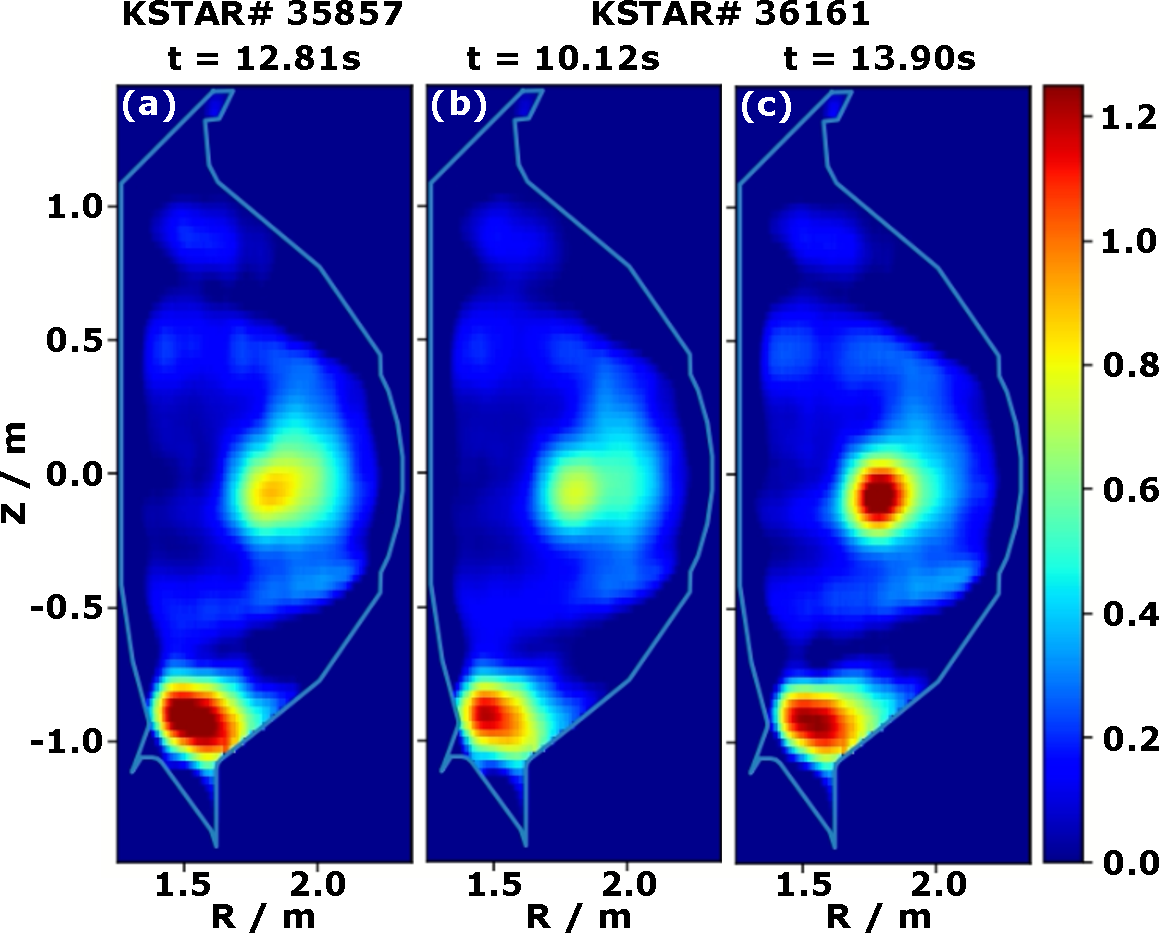
\includegraphics[width=\linewidth]{figures/Prad_2D.pdf}
 \caption{
KSTAR \ac{IRVB} measured radiated power density (a.u.) inverted into 2D cross-section.
(a) KSTAR \# 35857 at 12.81s at the peak of total radiated power.
(b) KSTAR \# 36161 at 10.12s before  the second impulse of gas between 10.8s to 12s.
(c) KSTAR \# 36161 at 13.90 after the last gas impulse.
}
\label{fig:prad_2d}
\end{figure}

Utilizing the controllers tuned in Sec.\ref{sec:sysid}, we attempted detachment control experiments.
First, we used \Afrac controller in KSTAR \# 35857 with results shown in Fig.\ref{fig:detctrl_afrac}.
As can be seen in Fig.\ref{fig:detctrl_afrac}a, the strike point remained within the realtime Langmuir probe array giving validity to the \Afrac signal shown in Fig.\ref{fig:detctrl_afrac}b.
Here, we can see that the controller was successful in closely following the target provided to it completing the pre-programmed shot length to the end.
It is also evident that the aggressive control strategy was good and did not result in any long sustained oscillations while providing a quick response to the changing target value.
From 8s to 10s, it can be seen that the injected N$_2$ was just enough to ramp down the measured \Afrac with the same slope.
The accumulated offset from the target eventually caused the integral term to send a brief impulse of nitrogen near 9.8s and then the controller futher converged with the target value.
For the rest of the shot, small nitrogen puffs were required to correct the drifting \Afrac and keep it on the target.
The total radiated power from the plasma as measured by KSTAR \ac{IRVB} remained below 3.5 MW and as can be seen in Fig.\ref{fig:prad_2d}a (snapshot taken at around the time of maximum radiation), the majority of the radiation was coming from the divertor region and the core region was not loosing power through radiation.
This further validated, that \Afrac controller strategy first devised in Ref.\cite{Eldon_2022_PPCF} is a viable option for detachment control even with Tungsten divertor in KSTAR.

Since \Afrac controller has been demonstrated in the past as well, we decided to utilize remaining alloted runtime on KSTAR to test the DivControlNN prototype-based controller.
Fig.\ref{fig:detctrl_sm} shows the results from shot \# 36161 where we deployed this controller.
An immediate issue was seen with DivControlNN output that the intial heat flux calculation had a different starting value than what we saw in reference shots and system identification shot \# 35854.
Because of this, when the controller turned on at 7.5s, the large error resulted in railing of gas command output which caused too much N$_2$ injected into the system.
While this quickly brought down the measured signal, it also resulted in an overshoot.
In the next rampdown of target from 10.5s to 11.5s, more impurity was injected as we tuned an aggresive controller.
It can be seen from \Afrac in Fig.\ref{fig:detctrl_sm}d that the system reached into deep detachment by this point and the ion saturation current measurements (Fig.\ref{fig:detctrl_sm}a) became unreliable beyond 11s.
In post-analysis of IRVB inverted data as shown in Fig.\ref{fig:prad_2d}, we can see that the core started radiating a lot of power after the last railed impulse of gas input between 10.8s to 12s.
This perhaps caused enough cooling of the core and the cross-drift of power into \ac{SOL} region reduced.
This mightb be why the heat flux (Fig.\ref{fig:detctrl_sm}b) did not naturally recover even when the target was lifted up between 13s to 15s.
There is no surprise with the fact that setting target values for an uncalibrated output is not always deterministic and would cause issues like we faced.

Post-shot data analysis discovered further issues in our operation of the DivControlNN model.
The impurity fraction calculation as mentioned in \ref{sec:control_variables} malfunctioned and sent a constant zero input to the model.
Thus the model was unable to respond to large amounts of impurity that were injected into the system and was only relying on data from line integrated core electron density and plasma current as realtime inputs.
In full carbon machine tests, it has been seen in the past\needcite that deuterium alone is sufficient to attain detachment as enough wall sourced intrinsic carbon impurity exists in the plasma during a campaign.
This might have been the case in shot \# 36161 as well, that even though impurity was seeded mostly as a feedback to observed electron density with a largely constant input power, the controller mostly worked initially as N$_2$ has similar radiation loss profile as carbon.
However, once the injected amount of nitrogen was beyond what the UEDGE simulation could assume background intrisic carbon to be, the relationship broke down and thus the control is not very good beyond 11s.
Despite these limitations, this preliminary test sheds light on the potential of using such a surrogate model based controller for detachment control in future reactors.